\documentclass[12pt, titlepage]{article}

\usepackage{booktabs}
\usepackage{tabularx}
\usepackage{hyperref}
\hypersetup{
    colorlinks,
    citecolor=black,
    filecolor=black,
    linkcolor=red,
    urlcolor=blue
}
\usepackage[round]{natbib}
\usepackage{float}
\usepackage{graphicx} 
\usepackage{array}
\usepackage{booktabs} 
\usepackage{longtable}

%% Comments

\usepackage{color}

\newif\ifcomments\commentstrue %displays comments
%\newif\ifcomments\commentsfalse %so that comments do not display

\ifcomments
\newcommand{\authornote}[3]{\textcolor{#1}{[#3 ---#2]}}
\newcommand{\todo}[1]{\textcolor{red}{[TODO: #1]}}
\else
\newcommand{\authornote}[3]{}
\newcommand{\todo}[1]{}
\fi

\newcommand{\wss}[1]{\authornote{blue}{SS}{#1}} 
\newcommand{\plt}[1]{\authornote{magenta}{TPLT}{#1}} %For explanation of the template
\newcommand{\an}[1]{\authornote{cyan}{Author}{#1}}

%% Common Parts

\newcommand{\progname}{PCD: Partially Covered Detection of Obscured People using Point Cloud Data} % PUT YOUR PROGRAM NAME HERE
\newcommand{\authname}{Team \#14, PCD
\\ Tarnveer Takhtar
\\ Matthew Bradbury
\\ Harman Bassi
\\ Kyen So} % AUTHOR NAMES                  

\usepackage{hyperref}
    \hypersetup{colorlinks=true, linkcolor=blue, citecolor=blue, filecolor=blue,
                urlcolor=blue, unicode=false}
    \urlstyle{same}

\usepackage{indentfirst}                              


\begin{document}

\title{Verification and Validation Report: \progname} 
\author{\authname}
\date{\today}
	
\maketitle

\pagenumbering{roman}

\section{Revision History}

\begin{tabularx}{\textwidth}{p{3cm}p{2cm}X}
\toprule {\bf Date} & {\bf Version} & {\bf Notes}\\
\midrule
2025-03-10 & 1.0 & Notes\\
April 2, 2025 & 2.0 & \href{https://github.com/takhtart/PCD/issues/118}{Revision 1}\\
April 2, 2025 & 2.0 & \href{https://github.com/takhtart/PCD/issues/119}{Revision 1}\\
April 3, 2025 & 2.0 & \href{https://github.com/takhtart/PCD/issues/123}{Revision 1}\\
April 4, 2025 & 2.0 & \href{https://github.com/takhtart/PCD/issues/122}{Revision 1}\\
April 4, 2025 & 2.0 & \href{https://github.com/takhtart/PCD/issues/124}{Revision 1}\\
\bottomrule
\end{tabularx}

~\newpage

\section{Symbols, Abbreviations and Acronyms}

\renewcommand{\arraystretch}{1.2}
\begin{tabular}{l l} 
  \toprule		
  \textbf{symbol} & \textbf{description}\\
  \midrule 
  T & Test\\
  N/I & Not Implemented\\
  \bottomrule
\end{tabular}\\

\newpage

\tableofcontents

\listoftables %if appropriate

\listoffigures %if appropriate

\newpage

\pagenumbering{arabic}

This document outlines the results and analysis of executing our VnV plan. Included below is a brief summary of each Functional, Non-functional, and Unit test, along with a description of their expected vs actual results. Provided with these results is the insight gained on the system that each tests highlights. "N/I" will be used for tests that have not yet been implemented.  

\section{Functional Requirements Evaluation}

\subsection{Human Detection Testing}
The following section covers the functional tests related to human detection given different coverage levels.
\begin{table}[H] % Force table to stay here
  \centering
  \renewcommand{\arraystretch}{1.4} % Adjust row height for better readability
  \resizebox{\textwidth}{!}{ % Ensures table fits within text width
  \begin{tabular}{|p{1.5cm}|p{2.5cm}|p{3cm}|p{4cm}|p{4cm}|p{1.8cm}|}
      \hline
      \textbf{ID} & \textbf{Type} & \textbf{Input} & \textbf{Expected Result} & \textbf{Actual Result} & \textbf{Pass/Fail} \\
      \hline
      FT11 & Manual & \raggedright Realtime PCD from Kinect & \raggedright Software recognizes that there is a human in frame in real-time & \raggedright Software recognizes that there is a human in frame in real-time & Pass \\
      \hline
      \multicolumn{6}{|p{\textwidth}|}{\raggedright \textbf{Description:} A pass in this test case would mean that our software has a strong enough foundation such that we can continue to refine towards more complicated test cases in the real-time environment. During our actual test, our software was able to first recognize that there was no human in frame. Then, once a human enters the frame, our software is able to cluster the human in real-time. This aligns with our expected results, thus, we consider this test a pass.} \\
      \hline
      FT12 & Manual & \raggedright Realtime PCD from Kinect & \raggedright Software recognizes that the human upper body is in frame in real-time & \raggedright Software recognizes that the human upper body is in frame in real-time & Pass \\
      \hline
      \multicolumn{6}{|p{\textwidth}|}{\raggedright \textbf{Description:} A pass in this test case would mean that the software has been able to recognize a human just by the upper body. In the actual test, the software was first able to recognize no one in frame. Then, when the human enters the frame, the software is able to pick up the upper body of the human. This aligns with the expected results, thus, we consider this a passing result.} \\
      \hline
      FT13 & Manual & \raggedright Realtime PCD from Kinect & \raggedright Software recognizes that there are two humans in frame in real time & \raggedright Software recognizes that there is 1 human in frame despite 2 people being in frame & Fail \\
      \hline
      \multicolumn{6}{|p{\textwidth}|}{\raggedright \textbf{Description:} A pass in this test case would mean that our software has the capability of detecting multiple people at once and distinguishing them between each other. This is very important for future use cases of our product where more than one person can appear in frame. During our actual test, our software was able to create two separate clusters for the two people in frame while they have some distance between them. However, as two people got closer together, our software began to cluster both people together. This does not align with our expected results, thus, we consider this test a fail.} \\
      \hline
      FT14 & Manual & \raggedright Realtime PCD from Kinect & \raggedright Software recognizes that there is a human within frame behind the object & \raggedright Software recognizes that there is a human within frame behind the object & Pass \\
      \hline
      \multicolumn{6}{|p{\textwidth}|}{\raggedright \textbf{Description:} A pass in this test case would mean that the software is able to determine that it is able to accomplish partially covered human detection. This is very important for future use cases of our product where a person is hidden behind an object in frame. During the actual test, when the human stands up from behind the object the software is able to outline the human cluster that it is able to detect within the frame. Thus, this test is a success showing that human detection of hidden objects is possible.} \\
      \hline
  \end{tabular}
  }
\end{table}

\begin{table}[H] % Force table to stay here
  \centering
  \renewcommand{\arraystretch}{1.4} % Adjust row height for better readability
  \resizebox{\textwidth}{!}{ % Ensures table fits within text width
  \begin{tabular}{|p{1.5cm}|p{2.5cm}|p{3cm}|p{4cm}|p{4cm}|p{1.8cm}|}
    \hline
      FT15 & Manual & \raggedright .pcd file containing the full-body of a human unobstructed by any objects & \raggedright Software recognizes that there is a human & \raggedright Software recognizes that there is a human & Pass \\
      \hline
      \multicolumn{6}{|p{\textwidth}|}{\raggedright \textbf{Description:} A pass in this test case would mean that our software has a strong enough foundation such that we can continue to refine towards more complicated test cases in an offline environment. During our actual test, we uploaded the test .pcd file and observed that our software correctly clustered the expected areas in the point cloud correctly which is where the human is located. Since our test aligns with our expected results, we consider this test a pass.} \\
      \hline
      FT16 & Manual & \raggedright .pcd file containing only the upper body of a human unobstructed by any objects & \raggedright Software recognizes that the human upper body is in frame & \raggedright Software recognizes that the human upper body is in frame & Pass \\
      \hline
      \multicolumn{6}{|p{\textwidth}|}{\raggedright \textbf{Description:} A pass in this test case would mean that the software has been able to recognize a human just by the upper body in an offline file. In the actual test, when the .pcd file is submitted the software is able to pick up the upper body of the human. This aligns with the expected results, thus, we consider this a passing result.} \\
      \hline
      FT17 & Manual & \raggedright .pcd file containing 2 humans with one human partially covering the other. & \raggedright Software recognizes that there are two humans in frame & \raggedright Software recognizes that there is 1 human in frame despite 2 people being in frame & Fail \\
      \hline
      \multicolumn{6}{|p{\textwidth}|}{\raggedright \textbf{Description:} A pass in this test would mean that our software has the capability of detecting multiple people at once and distinguishing them between each other in an offline environment. During our actual test, we uploaded the test .pcd file and observed that our software incorrectly clustered our two humans together as one cluster due to them being positioned too close together. This does not align with the expected results, thus, we consider this test a fail.} \\
      \hline
      FT18 & Manual & \raggedright .pcd file containing a human who is partially covered by an Object (table) & \raggedright Software recognizes that there is a human within frame behind the object & \raggedright Software recognizes that there is a human within frame behind the object & Pass \\
      \hline
      \multicolumn{6}{|p{\textwidth}|}{\raggedright \textbf{Description:} A pass in this test case would mean that the software is able to determine that it is able to accomplish partially covered human detection within a given .pcd file. This is very important for future use cases of our product where a person is hidden behind an object in frame. During the actual test, the file is uploaded and the software is able to detect the human standing behind the object. Thus, this test is a success showing that human detection of hidden objects is possible.} \\
      \hline
    \end{tabular}
    }
  \end{table}
\subsection{Location Prediction Test} \label{FT21} \label{FT24}
The following section covers the functional tests related to predicting the location of obscured segments.
\begin{table}[H] % Force table to stay here
  \centering
  \renewcommand{\arraystretch}{1.4} % Adjust row height for better readability
  \resizebox{\textwidth}{!}{ % Ensures table fits within text width
  \begin{tabular}{|p{2cm}|p{2.5cm}|p{3cm}|p{4cm}|p{4cm}|p{1.8cm}|} 
      \hline
      \textbf{ID} & \textbf{Type} & \textbf{Input} & \textbf{Expected Result} & \textbf{Actual Result} & \textbf{Pass/Fail} \\
      \hline
      FT21 & Manual & \raggedright Realtime PCD from Kinect \par & \raggedright A box drawn outwards to where the person is standing \par & A box drawn away from the hand at the center off to the end of the cloud showing the human outside of frame. & Pass \\
      \hline
      \multicolumn{6}{|p{\textwidth}|}{\raggedright \textbf{Description:} A pass in this test would indicate that the software is able to detect the approximate location of the person if they are partially out of frame. This is important as it shows that the location estimation is able to determine if the human is partially out of the scene. The actual test resulted in the box being drawn around the center of the person out of the point cloud a bit to showcase that they are partially out of frame. Thus, the test is a pass meaning that the software is able to know when the human is out of the screen. \par} \\
      \hline
      FT22 & Manual & \raggedright Realtime PCD from Kinect \par & \raggedright A box showing where the human's legs would be. \par & A box encompassing the human, drawing the box to where the legs should be as well. & Pass \\
      \hline
      \multicolumn{6}{|p{\textwidth}|}{\raggedright \textbf{Description:} A pass in this test would indicate that the software is able to detect people based of the given points and is able to use that to estimate the general location of where the human should be. In this specific test case the software draws a box around the human body and predicts where the legs of the body should be. This is seen in the actual tesing as well. Thus, proving that the software is able to successful predict the general location of the legs and not visble area of the human.  \par} \\
      \hline
  \end{tabular}
  }
\end{table}

\begin{table}[H] % Force table to stay here
  \centering
  \renewcommand{\arraystretch}{1.4} % Adjust row height for better readability
  \resizebox{\textwidth}{!}{ % Ensures table fits within text width
  \begin{tabular}{|p{2cm}|p{2.5cm}|p{3cm}|p{4cm}|p{4cm}|p{1.8cm}|} 
      \hline
      FT23 & Manual & \raggedright .pcd file containing a hand of a human outside the frame \par & \raggedright A box drawn outwards to where the person is standing \par & A box drawn away from the hand at the center off to the end of the cloud showing the human outside of frame. & Pass \\
      \hline
      \multicolumn{6}{|p{\textwidth}|}{\raggedright \textbf{Description:} A pass in this test would indicate that the software is able to detect the approximate location of the person if they are partially out of frame given a .pcd frame. This is important as it shows that the location estimation is able to determine if the human is partially out of the scene. The actual test had the submission of the file with this scenario and resulted in the box being drawn around the center of the person out of the point cloud a bit to showcase that they are partially out of frame. Thus, the test is a pass meaning that the software is able to know when the human is out of the screen. \par} \\
      \hline
      FT24 & Manual & \raggedright .pcd file containing a human who’s upper body is only visible \par & \raggedright A box showing where the human's legs would be. \par & A box drawn away from the hand at the center off to the end of the cloud showing the human outside of frame. & Pass \\
      \hline
      \multicolumn{6}{|p{\textwidth}|}{\raggedright \textbf{Description:} A pass in this test would indicate that the software is able to detect people based of the uploaded .pcd w and is able to use that to estimate the human. In the actual test has the user upload a .pcd and the software draws a box around the human body and where the legs of the body should be. Thus, proving that the software is able to successful predict the not visble area of the human. \par} \\
      \hline
  \end{tabular}
  }
\end{table}


\subsection{Offline Processing}
The following section covers the functional tests related to the offline processing of files.
\begin{table}[H] % Force table to stay here
  \centering
  \renewcommand{\arraystretch}{1.4} % Adjust row height for better readability
  \resizebox{\textwidth}{!}{ % Ensures table fits within text width
  \begin{tabular}{|p{1.5cm}|p{2.5cm}|p{3cm}|p{4cm}|p{4cm}|p{1.8cm}|} 
      \hline
      \textbf{ID} & \textbf{Type} & \textbf{Input} & \textbf{Expected Result} & \textbf{Actual Result} & \textbf{Pass/Fail} \\
      \hline
      FT31 & Automated & \raggedright Four not valid .pcd file and one valid .pcd file \par & \raggedright Software returns that the .pcd file is not valid \par & \raggedright Software returns that the .pcd file is not valid \par & Pass \\
      \hline
      \multicolumn{6}{|p{\textwidth}|}{\raggedright \textbf{Description:} A pass in this test would mean that our software is able to detect and run only the valid .pcd file. The actual results of this test were a pass because the software was able to return a catch error on the invalid files and run the valid file. Thus, the test is a pass meaning offline files can be properly handled by the offline .pcd reader. \par} \\
      \hline
      FT32 & Automated & \raggedright .jpg file \par & \raggedright Software returns incorrect format message for 4 / 5 files and accepts the 1 .pcd file \par & \raggedright Software returns incorrect format message for 4 / 5 files and accepts the 1 .pcd file \par & Pass \\
      \hline
      \multicolumn{6}{|p{\textwidth}|}{\raggedright \textbf{Description:} A pass in this test would mean that our software is able to identify if the user uploaded a file with the incorrect file format (one that isn’t .pcd) and notify the user accordingly. In the actual test, we ran our automated test which is set up to automatically upload 5 files (4 .jpg files and 1 .pcd). The software was able to identify that 4 of the 5 files were invalid meaning that it is able to reliably check for incorrect file formats. Since the test results align with the expected results, we consider this test a pass. \par} \\
      \hline
  \end{tabular}
  }
\end{table}


\subsection{Body Pose Variation Handling}
The following section covers the functional tests related to human detection give a dynamic set of poses.
\begin{table}[H] % Force table to stay here
  \centering
  \renewcommand{\arraystretch}{1.4} % Adjust row height for better readability
  \resizebox{\textwidth}{!}{ % Ensures table fits within text width
  \begin{tabular}{|p{1.5cm}|p{2.5cm}|p{3cm}|p{4cm}|p{4cm}|p{1.8cm}|} 
      \hline
      \textbf{ID} & \textbf{Type} & \textbf{Input} & \textbf{Expected Result} & \textbf{Actual Result} & \textbf{Pass/Fail} \\
      \hline
      FT41 \label{FT41} & Manual & \raggedright Realtime PCD from Kinect \par & \raggedright The outline of the human should be relatively the same when the face away from the camera \par & \raggedright The software is able to still detect the human based off the hand skin points \par & Pass \\
      \hline
      \multicolumn{6}{|p{\textwidth}|}{\raggedright \textbf{Description:} The test is a pass when the software is able to detect a person even if their face is hidden, but hands still visible. When running this test, when the human turned away from the sensor the software was still able to detect the human. Thus, the test was a pass showing that even if the face of the person is not in frame it is still able to detect the human. \par} \\
      \hline
      FT42 \label{FT42} & Manual & \raggedright Realtime PCD from Kinect \par & \raggedright The software is able to identify the human even if they are sitting. \par & \raggedright When the software was run, the software outlined the human sitting. \par & Fail \\
      \hline
      \multicolumn{6}{|p{\textwidth}|}{\raggedright \textbf{Description:} A pass in this test would mean that our software is able to identify people in a variety of poses rather than just standing. In the actual test, we position a person sitting in a chair whilst facing the camera. Although the software was able to correctly cluster the person while they are sitting, it incorrectly clusters the chair along with the person in the same cluster. This does not align with the expected results, thus, we consider this test a fail. \par} \\
      \hline
      FT43 \label{FT43} & Manual & \raggedright Realtime PCD from Kinect \par & \raggedright The software is able to identify the human every time the face comes into frame. \par & \raggedright When ran, the software is able to identify the human when the face comes in frame. \par & Pass \\
      \hline
      \multicolumn{6}{|p{\textwidth}|}{\raggedright \textbf{Description:} The test is a pass if the system is able to detect and outline a human if it is able to see the skin points from the face and detect the partial human. During the actual test, the software was able to notice the head bobbing in and out and was able to detect a human when the head was in frame. Therefore, proving the test to be a success shows that when the system is able to see a skin point it is able to successfully detect a human in frame. \par} \\
      \hline
  \end{tabular}
  }
\end{table}

\subsection{Integration with Kinect Sensor}
The following section covers the functional tests related to the connection and data transfer of the Kinect Sensor.
\begin{table}[H] % Force table to stay here
  \centering
  \renewcommand{\arraystretch}{1.4} % Adjust row height for better readability
  \resizebox{\textwidth}{!}{ % Ensures table fits within text width
  \begin{tabular}{|p{1.5cm}|p{2.5cm}|p{3cm}|p{4cm}|p{4cm}|p{1.8cm}|} 
      \hline
      \textbf{ID} & \textbf{Type} & \textbf{Input} & \textbf{Expected Result} & \textbf{Actual Result} & \textbf{Pass/Fail} \\
      \hline
      FT51 & Manual & \raggedright Disconnection and reconnection of Kinect \par & \raggedright The software does not crash, but freezes. \par & \raggedright When Kinect is disconnected the output freezes. \par & Pass \\
      \hline
      \multicolumn{6}{|p{\textwidth}|}{\raggedright \textbf{Description:} A pass in this test would mean that the software is able to properly determine if the Kinect sensor is no longer connected. During the actual test, the Kinect is disconnected and the software does not crash. Therefore, this is a successful test making sure that the software won’t crash. \par} \\
      \hline
      FT52 & Manual & \raggedright Realtime PCD from Kinect \par & \raggedright Our software visualizes a point cloud that is accurate to what the Kinect is capturing in real-time. \par & \raggedright Our software visualizes a point cloud that is accurate to what the Kinect is capturing in real-time. \par & Pass \\
      \hline
      \multicolumn{6}{|p{\textwidth}|}{\raggedright \textbf{Description:} A pass in this test would mean that our software is able to accurately convert the data that it receives from the Kinect to the point cloud format. During our actual test, we observed that the gestures we make in front of the Kinect sensor are accurately portrayed when visualizing the point cloud despite a slight time delay. Since the test results align with the expected results, we consider this test a pass. \par} \\
      \hline
  \end{tabular}
  }
\end{table}

\subsection{Realtime Processing}
The following section covers the non-functional tests related to performance metrics.
\begin{table}[H] % Force table to stay here
  \centering
  \renewcommand{\arraystretch}{1.4} % Adjust row height for better readability
  \resizebox{\textwidth}{!}{ % Ensures table fits within text width
  \begin{tabular}{|p{1.5cm}|p{2.5cm}|p{3cm}|p{4cm}|p{4cm}|p{1.8cm}|} 
      \hline
      \textbf{ID} & \textbf{Type} & \textbf{Input} & \textbf{Expected Result} & \textbf{Actual Result} & \textbf{Pass/Fail} \\
      \hline
      NFT11 & Manual & \raggedright Realtime PCD from Kinect \par & \raggedright Software is able to update and produce an outline of the head within 1s each time the head pokes out \par & \raggedright Software is able to update and produce an outline of the head after approximately 642 ms (averaged out of 10 runs) \par & Pass \\
      \hline
      \multicolumn{6}{|p{\textwidth}|}{\raggedright \textbf{Description:} A pass in this test means that our software meets the non-functional requirement of being a real-time system. During our test, our tester was able to measure a less than a second delay for each of the ten attempts we did. The measurement of the time delay averaged out to around 642ms. Since the test results align with the expected results, we consider this test a pass. \par} \\
      \hline
  \end{tabular}
  }
\end{table}


\section{Non-Functional Requirements Evaluation}

\subsection{Usability}
The following section covers the non-functional tests related to usability metrics. The user in this scenario has no idea how to run the software.
\begin{table}[H] % Force table to stay here
  \centering
  \renewcommand{\arraystretch}{1.4} % Adjust row height for better readability
  \resizebox{\textwidth}{!}{ % Ensures table fits within text width
  \begin{tabular}{|p{1.5cm}|p{2.5cm}|p{3cm}|p{4cm}|p{4cm}|p{1.8cm}|} 
      \hline
      \textbf{ID} & \textbf{Type} & \textbf{Input} & \textbf{Expected Result} & \textbf{Actual Result} & \textbf{Pass/Fail} \\
      \hline
      NFT11 & Manual & \raggedright The user is given the Setup.md (link), a laptop without any necessary downloads, and the Kinect. \par & \raggedright User is able to set up on the laptop and run the software in the live scenario using the Kinect. This is all expected to take 10-15 minutes without download times included.\par & \raggedright The user takes approximately 12 minutes to set up and get it all running. \par & Pass \\
      \hline
      \multicolumn{6}{|p{\textwidth}|}{\raggedright \textbf{Description:} A pass in this test means that our software meets the non-functional requirement of being a usable system. During our test, the user did not struggle with the set up and followed along easily with the set up documentation. They completed within the time frame given and did not have any questions during the test either. Since the test results align with the expected results, we consider this test a pass. \par} \\
      \hline
      NFT12 \label{NFT12} & Manual & \raggedright A .pcd file that user is uploading \par & \raggedright User is able to upload a .pcd file without any issues and have the expected outcome displayed on the screen \par & \raggedright User had zero issues and did what was expected. The user was able to run offline mode and upload a .pcd file. \par & Pass \\
      \hline
      \multicolumn{6}{|p{\textwidth}|}{\raggedright \textbf{Description:} A pass in this test means that our software meets the non-functional requirement of being a usable system. During our test, the user had zero issue uploading a file showing that the current proccess is straightforward, even when there is zero knowledge about the system. Since the test results align with the expected results, we consider this test a pass. \par} \\
      \hline
  \end{tabular}
  }
\end{table}
		
\subsection{Reliability}
The following section covers the non-functional tests related to reliability requirements.
\begin{table}[H] % Force table to stay here
  \centering
  \renewcommand{\arraystretch}{1.4} % Adjust row height for better readability
  \resizebox{\textwidth}{!}{ % Ensures table fits within text width
  \begin{tabular}{|p{1.5cm}|p{2.5cm}|p{3cm}|p{4cm}|p{4cm}|p{1.8cm}|} 
      \hline
      \textbf{ID} & \textbf{Type} & \textbf{Input} & \textbf{Expected Result} & \textbf{Actual Result} & \textbf{Pass/Fail} \\
      \hline
      NFT21 & Automated & \raggedright .pcd file with an object partially obstructing a human \par & \raggedright Software is able to reliably produce a very similar cluster each time it runs and the difference should be less than 5-10\% compared to the original run. \par & \raggedright Software is able to reliably produce the same cluster each time it runs and the difference is 0\% compared to the original run. \par & Pass \\
      \hline
      \multicolumn{6}{|p{\textwidth}|}{\raggedright \textbf{Description:} A pass in this test means that our software meets the non-functional requirement of being reliable. During our test, our software was able to produce the exact same result for all 10 times the same file was uploaded to the software. Therefore, the difference between the original run and each subsequent run is 0\%. Since the test results align with the expected results, we consider this test a pass. \par} \\
      \hline
  \end{tabular}
  }
\end{table}

\subsection{Accuracy}
The following section covers the non-functional tests related to accuracy requirements.
\begin{table}[H] % Force table to stay here
  \centering
  \renewcommand{\arraystretch}{1.4} % Adjust row height for better readability
  \resizebox{\textwidth}{!}{ % Ensures table fits within text width
  \begin{tabular}{|p{1.5cm}|p{2.5cm}|p{3cm}|p{4cm}|p{4cm}|p{1.8cm}|} 
      \hline
      NFT31 & Manual & \raggedright Realtime PCD from Kinect \par & \raggedright An average score of 80 percent \par & \raggedright An average score of 86 percent \par & Pass \\
      \hline
      \multicolumn{6}{|p{\textwidth}|}{\raggedright \textbf{Description:} A pass in this test would be if the human outlined is outlined within a reasonable range to be considered part of the human (i.e., clothes or object being held). An average rating of 80 percent determines how accurate the software is from 1-10. When the test was run, the view deemed the test to pass at 86 percent. The main issues arose with holding a big object. The test is deemed a success. \par} \\
      \hline
  \end{tabular}
  }
\end{table}

\section{Unit Testing}

\begin{table}[H] % Force table to stay here
  \centering
  \renewcommand{\arraystretch}{1.4} % Adjust row height for better readability
  \resizebox{\textwidth}{!}{ % Ensures table fits within text width
  \begin{tabular}{|p{1.5cm}|p{2.5cm}|p{3cm}|p{4cm}|p{4cm}|p{1.8cm}|}
      \hline
      \textbf{ID} & \textbf{Type} & \textbf{Input} & \textbf{Expected Result} & \textbf{Actual Result} & \textbf{Pass/Fail} \\
      \hline
      UT1 & Automated & \raggedright Sample PCL Point Cloud \par & \raggedright The RGB values, Depth Values, and Cloud Size are mapped correctly between file types. \par & \raggedright The RGB values, Depth Values, and Cloud Size are mapped correctly between file types. \par & Pass \\
      \hline
      \multicolumn{6}{|p{\textwidth}|}{\raggedright \textbf{Description:} ConvertPCLtoOpenCV: Converts a PCL Point Cloud to OpenCV Mat type for point cloud analysis using OpenCV. A pass means that the function correctly maps the Point Cloud values to OpenCV Mat type. The unit test passed successfully, verifying that the mapped values matched between the two types. \par} \\
      \hline
      UT2 & Automated & \raggedright Sample PCL cloud with a valid cluster \par & \raggedright The test should pass with the cluster being a valid cluster \par & \raggedright The test should pass with the cluster being a valid cluster  \par & Pass \\
      \hline
      \multicolumn{6}{|p{\textwidth}|}{\raggedright \textbf{Description:} valid$\_$cluster: The function needs to be able to ensure that the cluster is valid to allow for proper human detection to occur. A pass means that the function is able to determine that the cloud is valid and thus accepted. In this case the unit test pass, meaning that the valid$\_$cluster function can determine if the cluster presented is valid or not.  \par} \\
      \hline
      UT3 & Automated & \raggedright Sample PCL cloud with an invalid cluster \par & \raggedright The test should pass with the cluster being an invalid cluster \par & \raggedright The test should pass with the cluster being an invalid cluster \par & Pass \\
      \hline
      \multicolumn{6}{|p{\textwidth}|}{\raggedright \textbf{Description:} invalid$\_$cluster: The function needs to be able to ensure that the cluster is valid to allow for proper human detection to occur. A pass means that the function is able to determine that the cloud is invalid and thus rejected. In this case the unit test pass, meaning that the valid$\_$cluster function can determine if the cluster presented is valid or not. \par} \\
      \hline
  \end{tabular}
  }
\end{table}

\begin{table}[H] % Force table to stay here
  \centering
  \renewcommand{\arraystretch}{1.4} % Adjust row height for better readability
  \resizebox{\textwidth}{!}{ % Ensures table fits within text width
  \begin{tabular}{|p{1.5cm}|p{2.5cm}|p{3cm}|p{4cm}|p{4cm}|p{1.8cm}|}
      \hline
      UT4 & Automated & \raggedright Sample PCL cloud with predetermined points \par & \raggedright The number of PCL cloud points should be less than the original number of points (100) after the downsampling. \par & \raggedright The number of PCL cloud points should be less than the original number of points (100) after the downsampling.  \par & Pass \\
      \hline
      \multicolumn{6}{|p{\textwidth}|}{\raggedright \textbf{Description:} voxel$\_$downsampling: Runs the voxel downsampling to make sure the PCL cloud is downsamplied to make the cloud easier to processes. A pass means that the downsampling is correclty removing excess points to simplify the cloud. The unit test passed successfully, meaning that the fucntion is correclty downsampling the PCL cloud.   \par} \\
      \hline
      UT5 & Automated & \raggedright Sample PCL cloud with noise added \par & \raggedright The filtered cloud has points less than or equal to the original cloud.  \par & \raggedright There are less than or equal to 100 points in the filtered PCL cloud. \par & Pass \\
      \hline
      \multicolumn{6}{|p{\textwidth}|}{\raggedright \textbf{Description:} removeNoise: Runs a noise removal on the PCL cloud with the added noise points making sure that the number of points is equla to or less than the number of points in the cloud before the added noise. A pass that the function is able to correctly identify the noise added to the file and remove it leaving with a noise filtered PCL cloud with less than or equal to number of points as the original cloud. The Unit Test passed meaning the function is able to correctly identify the noise and removes it.  \par} \\
      \hline
  \end{tabular}
  }
\end{table}



\section{Changes Due to Testing}

After the Dr. Bone meeting, it was established that the human body parts would not need to be identified, which made the 3D Space Estimation testing unnecessary. This would mean that this test section would no longer be needed. But, the addition of a new functional requirement of location prediction would require some tests \hyperref[FT21]{FT21}-\hyperref[FT24]{FT24}. The location prediction is meant to predict where the human should be located based on the skin points detected. This now has four new tests, two for live and two for offline. The function has not yet been implemented for testing to occur.

Some of the body pose variation detection was altered slightly to match closer to the detection algorithm \hyperref[FT41]{FT41} - \hyperref[FT43]{FT43}. After the Dr. Bone meeting, it was determined to be a good idea to use skin points to determine a human in frame. These tests are now accounting for different body poses, but with human skin points being in frame.

After doing the \hyperref[NFT12]{NFT12}  test, even though the test was a success, the user was provided with the file to upload and so now in the command line the output also says the expected file time.


\section{Automated Testing}

The only automated testing present is the Unit Tests, which are run using CTest and GTest Suites.
		
\section{Trace to Requirements and Modules}		
See section G.4 in the \href{https://github.com/takhtart/PCD/blob/main/docs/SRS/SRS.pdf}{SRS report} for more information on the requirements. See section 7 in the \href{https://github.com/takhtart/PCD/blob/main/docs/Design/SoftArchitecture/MG.pdf}{Module Guide} for more information on the modules.

\begin{table}[H]

  \centering
  \caption{Module and Requirement Tracing}
  \begin{tabular}{|l|l|l|}
  \hline
  \textbf{Test ID} & \textbf{Requirement ID} & \textbf{Modules}\\
  \hline
  FT11 & F411 & M5, M6, M7, M8, M9\\
  \hline
  FT12 & F411 & M5, M6, M7, M8, M9\\
  \hline
  FT13 & F411 & M5, M6, M7, M8, M9\\
  \hline
  FT14 & F411 & M5, M6, M7, M8, M9\\
  \hline
  FT15 & F411 & M5, M6, M7, M8, M9\\
  \hline
  FT16 & F411 & M5, M6, M7, M8, M9\\
  \hline
  FT17 & F411 & M5, M6, M7, M8, M9\\
  \hline
  FT18 & F411 & M5, M6, M7, M8, M9\\
  \hline
  FT21 & F412 & M7, M11\\
  \hline
  FT22 & F412 & M7, M11\\
  \hline
  FT23& F412 & M7, M11\\
  \hline
  FT24 & F412 & M7, M11\\
  \hline
  FT31 & F413 & M4, M5, M6, M8, M9, M10, M11\\
  \hline
  FT32 & F413 & M4, M5, M6, M8, M9, M10, M11\\
  \hline
  FT41 & F414 & M4, M5, M6, M8, M9\\
  \hline
  FT42 & F414 & M4, M5, M6, M8, M9\\
  \hline
  FT43 & F414 & M4, M5, M6, M8, M9\\
  \hline
  FT51 & F415 & M1, M2\\
  \hline
  FT52 & F415 & M1, M2\\
  \hline
  NFT11 & NF431 & M1, M2, M9\\
  \hline
  NFT12 & NF432 & M5, M6, M7, M9\\
  \hline
  NFT13 & NF433 & M5, M6, M7\\
  \hline
  \end{tabular}
\end{table}

\section{Code Coverage Metrics}

The automated unit testing achieves 6\% line coverage. This is checked using CTest and OpenCPPCoverage Suites to acquire coverage results.\\
\\
OpenCPPCoverage Result:

\begin{figure}[h]
    \centering
    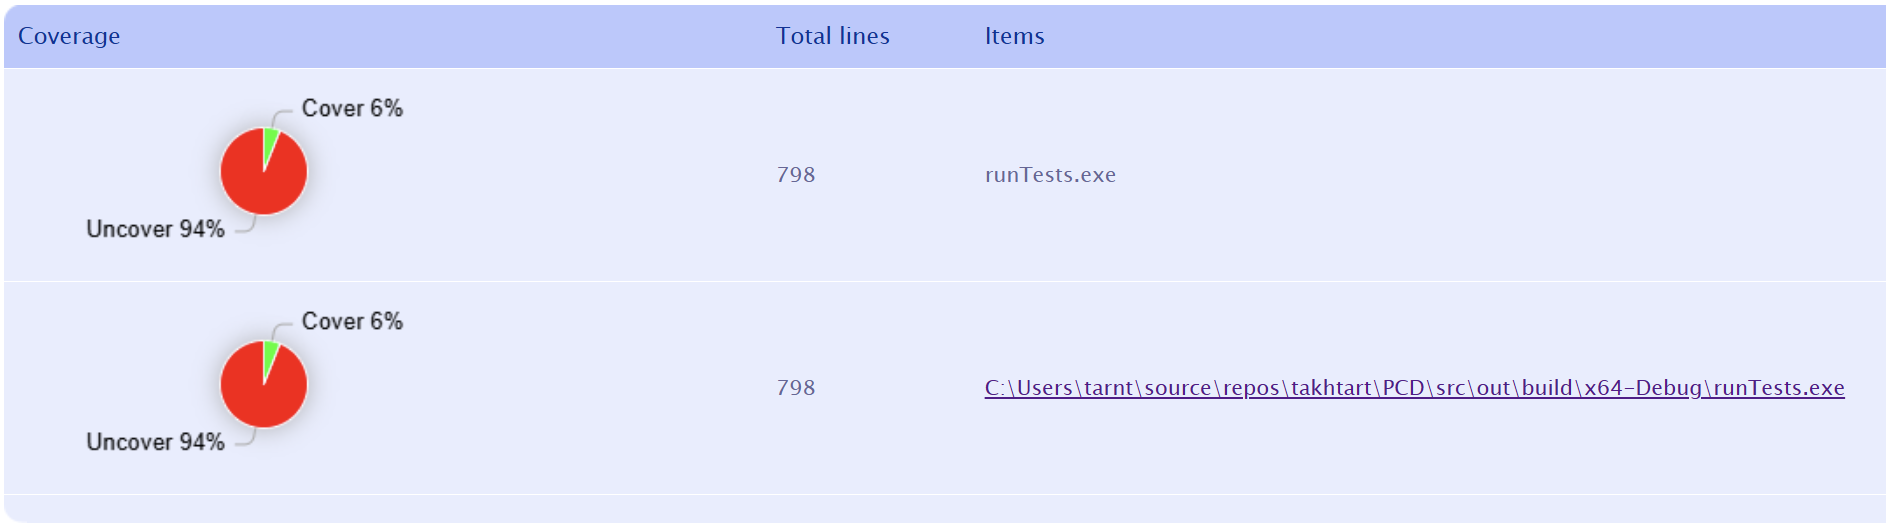
\includegraphics[width=1\textwidth]{Coverage.png} % Adjust width as needed
    \caption{OpenCPPCoverage Result}
    \label{fig:coverage}
\end{figure}

\bibliographystyle{plainnat}
\bibliography{../../refs/References}

\newpage{}
\section*{Appendix --- Reflection}

The information in this section will be used to evaluate the team members on the
graduate attribute of Reflection.

\begin{enumerate}
  \item What went well while writing this deliverable? \\
  \\
  When writing this deliverable, the sections that were very smooth were the ones that stemmed directly from the VnV plan. Those sections that went exactly as planned as the VnV Plan were very easy to translate to this report.
  \item What pain points did you experience during this deliverable, and how
    did you resolve them? \\
  \\
  A slight pain point that we did run into had to do with a change we received from Dr. Bone after Rev0. He proposed a change clarifying his vision for the project. This change caused one of our requirements to be completely reworked, changing the associated tests as well. We resolved this by simply moving back and rewriting the requirement, planned tests, and report tests that related to this requirement.
  \item Which parts of this document stemmed from speaking to your client(s) or
  a proxy (e.g. your peers)? Which ones were not, and why?\\
  \\
  The parts of the document that stemmed from speaking to our supervisor were the ones relating to the requirement mentioned in the above question. The rest of the requirements we generated previously based on the initial specification from Dr. Bone, which he checked and approved. The only new tests, that weren't described in the VnV Plan, were those related to the new reworked requirement stemming from Dr. Bone's feedback.
  \item In what ways was the Verification and Validation (VnV) Plan different
  from the activities that were actually conducted for VnV?  If there were
  differences, what changes required the modification in the plan?  Why did
  these changes occur?  Would you be able to anticipate these changes in future
  projects?  If there weren't any differences, how was your team able to clearly
  predict a feasible amount of effort and the right tasks needed to build the
  evidence that demonstrates the required quality?  (It is expected that most
  teams will have had to deviate from their original VnV Plan.) \\
  \\
  Aside from the changes mentioned in the previous question, we had to slightly tweak some of the test procedures initially proposed in the VnV Plan. In the beginning we weren't set on what method we were using for human detection and ended up trying a few different ways. The test procedures were initially written without any specific method in mind. Later on, after many meetings with Dr. Bone, we settled on a method that mainly uses skin point detection and region growing. Because of this method some of the test procedures didn't really make sense, namely any one that caused the person to maneuver into a position that hid all skin from the camera. The changes that this required was simply to move back to the VnV plan and tweak the procedure in such a way that kept the original intent of the test but made it feasible to test with our method of detection. Regarding these issues, I don't think we would be able to predict roadblocks like this in the future. The nature of these issues stem from explorations during development and would be difficult to account for prior.
\end{enumerate}

\end{document}